La société Let There Be Light (ou LTBL) est une société qui réalise des dispositifs interactifs pour l'événementiel, la communication et la culture.
Elle fut fondée en 2014 par Benjamin \bsc{Petit} et Antoine \bsc{Vanel} sous le nom de Beam'Art.
En 2016, elle change de nom et de statut pour devenir l'entreprise que l'on connaît aujourd'hui.
Actuellement, M. \bsc{Petit} en est le seul dirigeant et emploi 2 personnes.

\begin{description}
    \item[2012] Première fête des Lumières de Lyon dans le cadre d'une association avec un spectacle interactif nommé "Hypermétrope"
    \item[2014] Fondation de la société Beam'Art
    \item[2014] Installation interactive "Hi Striker" sur le palais de justice
    \item[2014] Mapping "TranJS" à Bernes
    \item[2015] Installation interactive "Lumibus" pour Keolis
    \item[2016] Changement de nom pour devenir Let There Be Light
    \item[2016] Participation à la création du showroom Pavillon de l'innovation pour Michelin
    \item[2017] Scénographie au Transbordeurs "DELete"
\end{description}

\subsection{Structure}

Let There Be Light est un partenaire de la société Vendredi 4.
Vendredi 4 est une société de communication spécialisée dans l'interaction.
Les contrats sont obtenus par Sylvie \bsc{Madamour}, la charte graphique du projet est alors composée par Vendredi 4.
LTBL intervient sur l'intégration de cette charte graphique dans les installations interactives dans des salons ou des showrooms.

Les équipes de Vendredi 4 et de LTBL sont assez réduites.
L'effectif de Vendredi 4 est de 3 employé quand LTBL compte un unique employé (Benjamin \bsc{Petit}) et deux consultants : Corentin \bsc{Limoge} et Alexander \bsc{Feller}.

\begin{figure}[h]
    \centering
    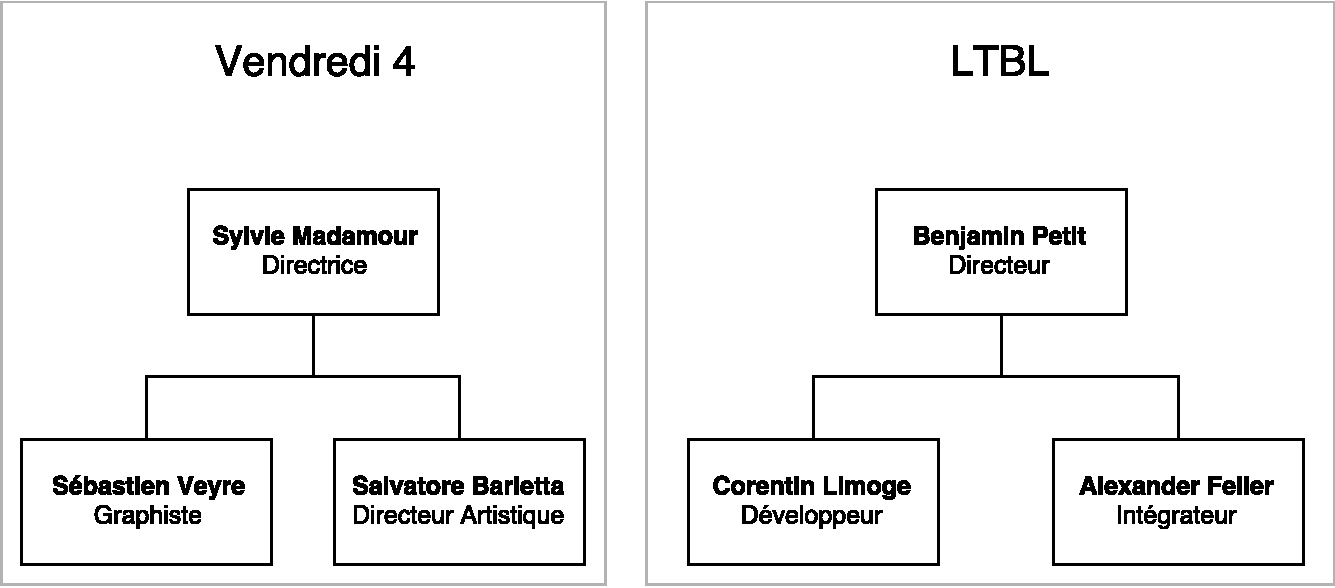
\includegraphics[scale=0.7]{img/Structure-LTBL.pdf}
    \caption{Structure de LTBL et Vendredi 4}
\end{figure}

Les deux entreprises sont très liées, elles partagent les mêmes locaux et communiquent beaucoup ensemble sur les projets en cours et à venir.

On retrouve alors Benjamin \bsc{Petit}, le gérant, et Corentin \bsc{Limoge} du côté LTBL.
Benjamin s'occupe des conseils et de la gestion de l'entreprise.
Il s'occupe aussi de l'aspect technique des installations par le choix des technologies de pointage et d'affichage.
Corentin est employé par LTBL, mais dispose d'un statut d'auto-entrepreneur, on peut alors le considérer comme un consultant.
Corentin est en charge du développement des applications qui seront exécutées sur les installations.

Du côté Vendredi 4, on retrouve Sylvie \bsc{Madamour}, la directrice, Salvatore \bsc{Barletta}, directeur artistique, et Sébastien \bsc{Veyre}, graphiste.
Sylvie est en charge des contrats, devis et de la communication avec les clients.
Salvatore est directeur artistique chez Vendredi 4, il s'occupe de concevoir et présenter les design des installations aux clients.
Sébastien est graphiste et est en charge de représenter les futures interfaces des installations, mais aussi de travailler sur des rendus en Motion Design\footnote{Une technique d'animation graphique ayant pour but de mettre en valeur le mouvement et l'animation.} Pour donner un premier aperçu de la future application pour les clients et les intégrateurs.

\subsection{Projets}

Les deux entreprises travaillent ensemble pour proposer des services suivants :

\begin{itemize}
    \item Conseils techniques
    \item Conseils en interaction
    \item Design graphique
    \item Développement d'applications interactives
    \item Installations
\end{itemize}

Ainsi, les deux entreprises peuvent suivre la production d'une application interactive de sa conception jusqu'à son installation.

\medskip

Les projets suivis par LTBL sont les suivants :

\paragraph{Dispositifs de présentation interactifs} le plus souvent utilisés dans les salons et showrooms, les dispositifs interactifs permettent une présentation des produits de manière esthétique.
L'objectif de LTBL est donc de concevoir cette installation.
Cela passe par la conception du système physique est des composants requis mais aussi par la conception et le développement de l'interface utilisateur qui doit être réactive et esthétique.
La majorité de ce type de projet est la présentation d'informations sur un produit sur un écran tactile

\paragraph{Vidéo Mapping} Le plus souvent présenté lors d'événements, le vidéo mapping consiste en la projection d'une image déformée sur une structure pouvant être un bâtiment ou une installation spécifique.
Cette image utilise une représentation de la structure pour se déformer et épouser sa forme lors de la projection.
Ce type d'installation permet, au travers de jeux de lumière et d'illusions, de donner vie à la structure ou au bâtiment.
On retrouve ce type d'installation à la fête des Lumières de Lyon par exemple.

\paragraph{Conseils techniques ou en interaction} Fort de son expérience dans le domaine de l'interactivité, LTBL peut aussi donner des conseils en interactivité dans le cadre de projets cités plus haut.

\paragraph{Fête des Lumières} La fête des Lumières est une manifestation Lyonnaise prenant place aux endroits importants de la ville.
Cette fête met en lumière de nombreuses installations lumineuses et interactives.
Chaque année, LTBL peut proposer un projet d'installation en rapport avec un bâtiment de la ville sur lequel s'installer.
Ce projet est alors évalué et est accepté ou non en fonction de la faisabilité, l'esthétique et le coût de l'installation.
La dernière fête des Lumières à laquelle a participé LTBL fut celle de 2015 avec une installation nommée "Lumibus".
Cette installation présentait un Bus muni de panneaux LED réagissant aux accélérations et freinages de celui-ci.
Les années précédentes, LTBL a aussi présenté Hi Striker, une installation reprenant le jeu de foire de la massue où les participants doivent taper le plus fort possible sur un capteur à l'aide d'une massue.
Plus la frappe est forte plus le bâtiment s'illumine.
Cette installation se trouvait au palais de justice.
Plus récemment, LTBL a participé à la fête des Lumières de Hong Kong avec un projet reprenant le même principe, mais en animant un dragon.

\begin{figure}[h]
    \centering
    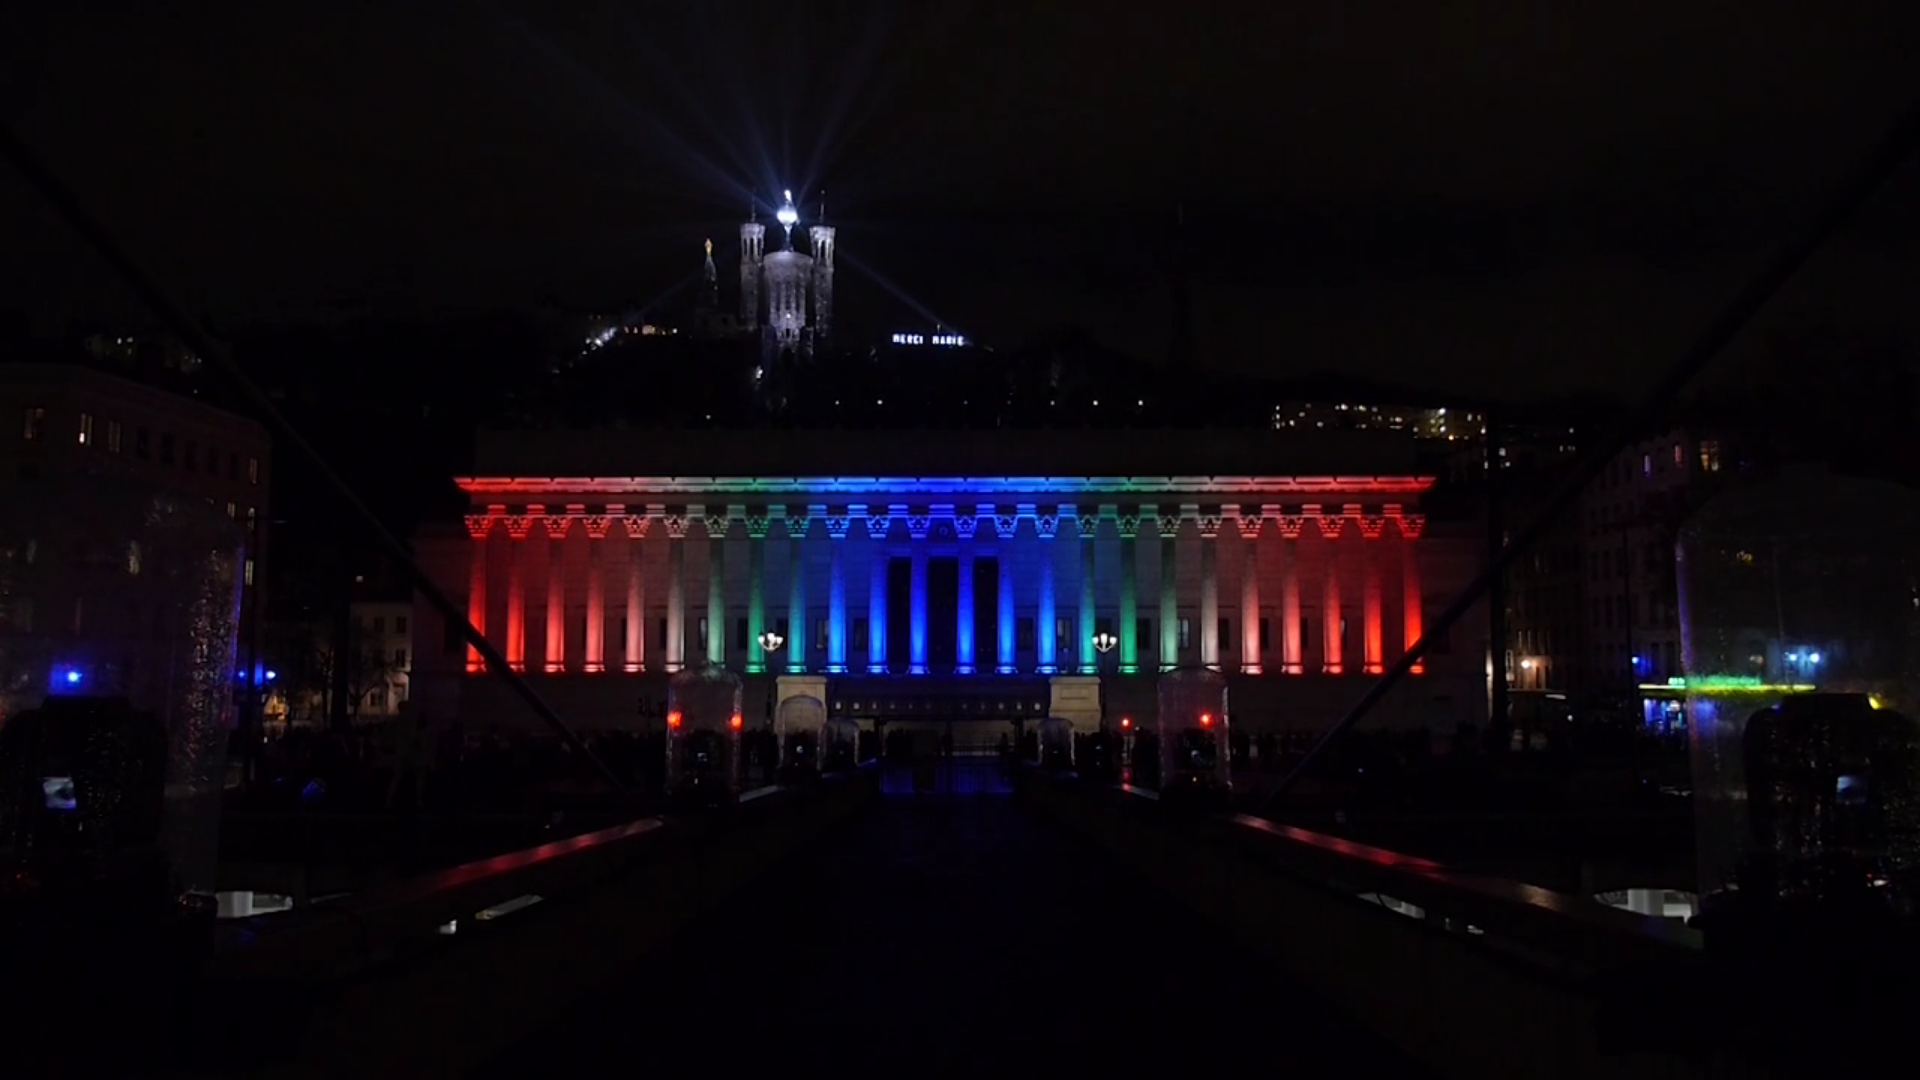
\includegraphics[scale=0.2]{img/hi-striker.png}
    \caption{L'installation "Hi Striker" à la fête des Lumières de Lyon}
\end{figure}


\begin{figure}[h]
    \centering
    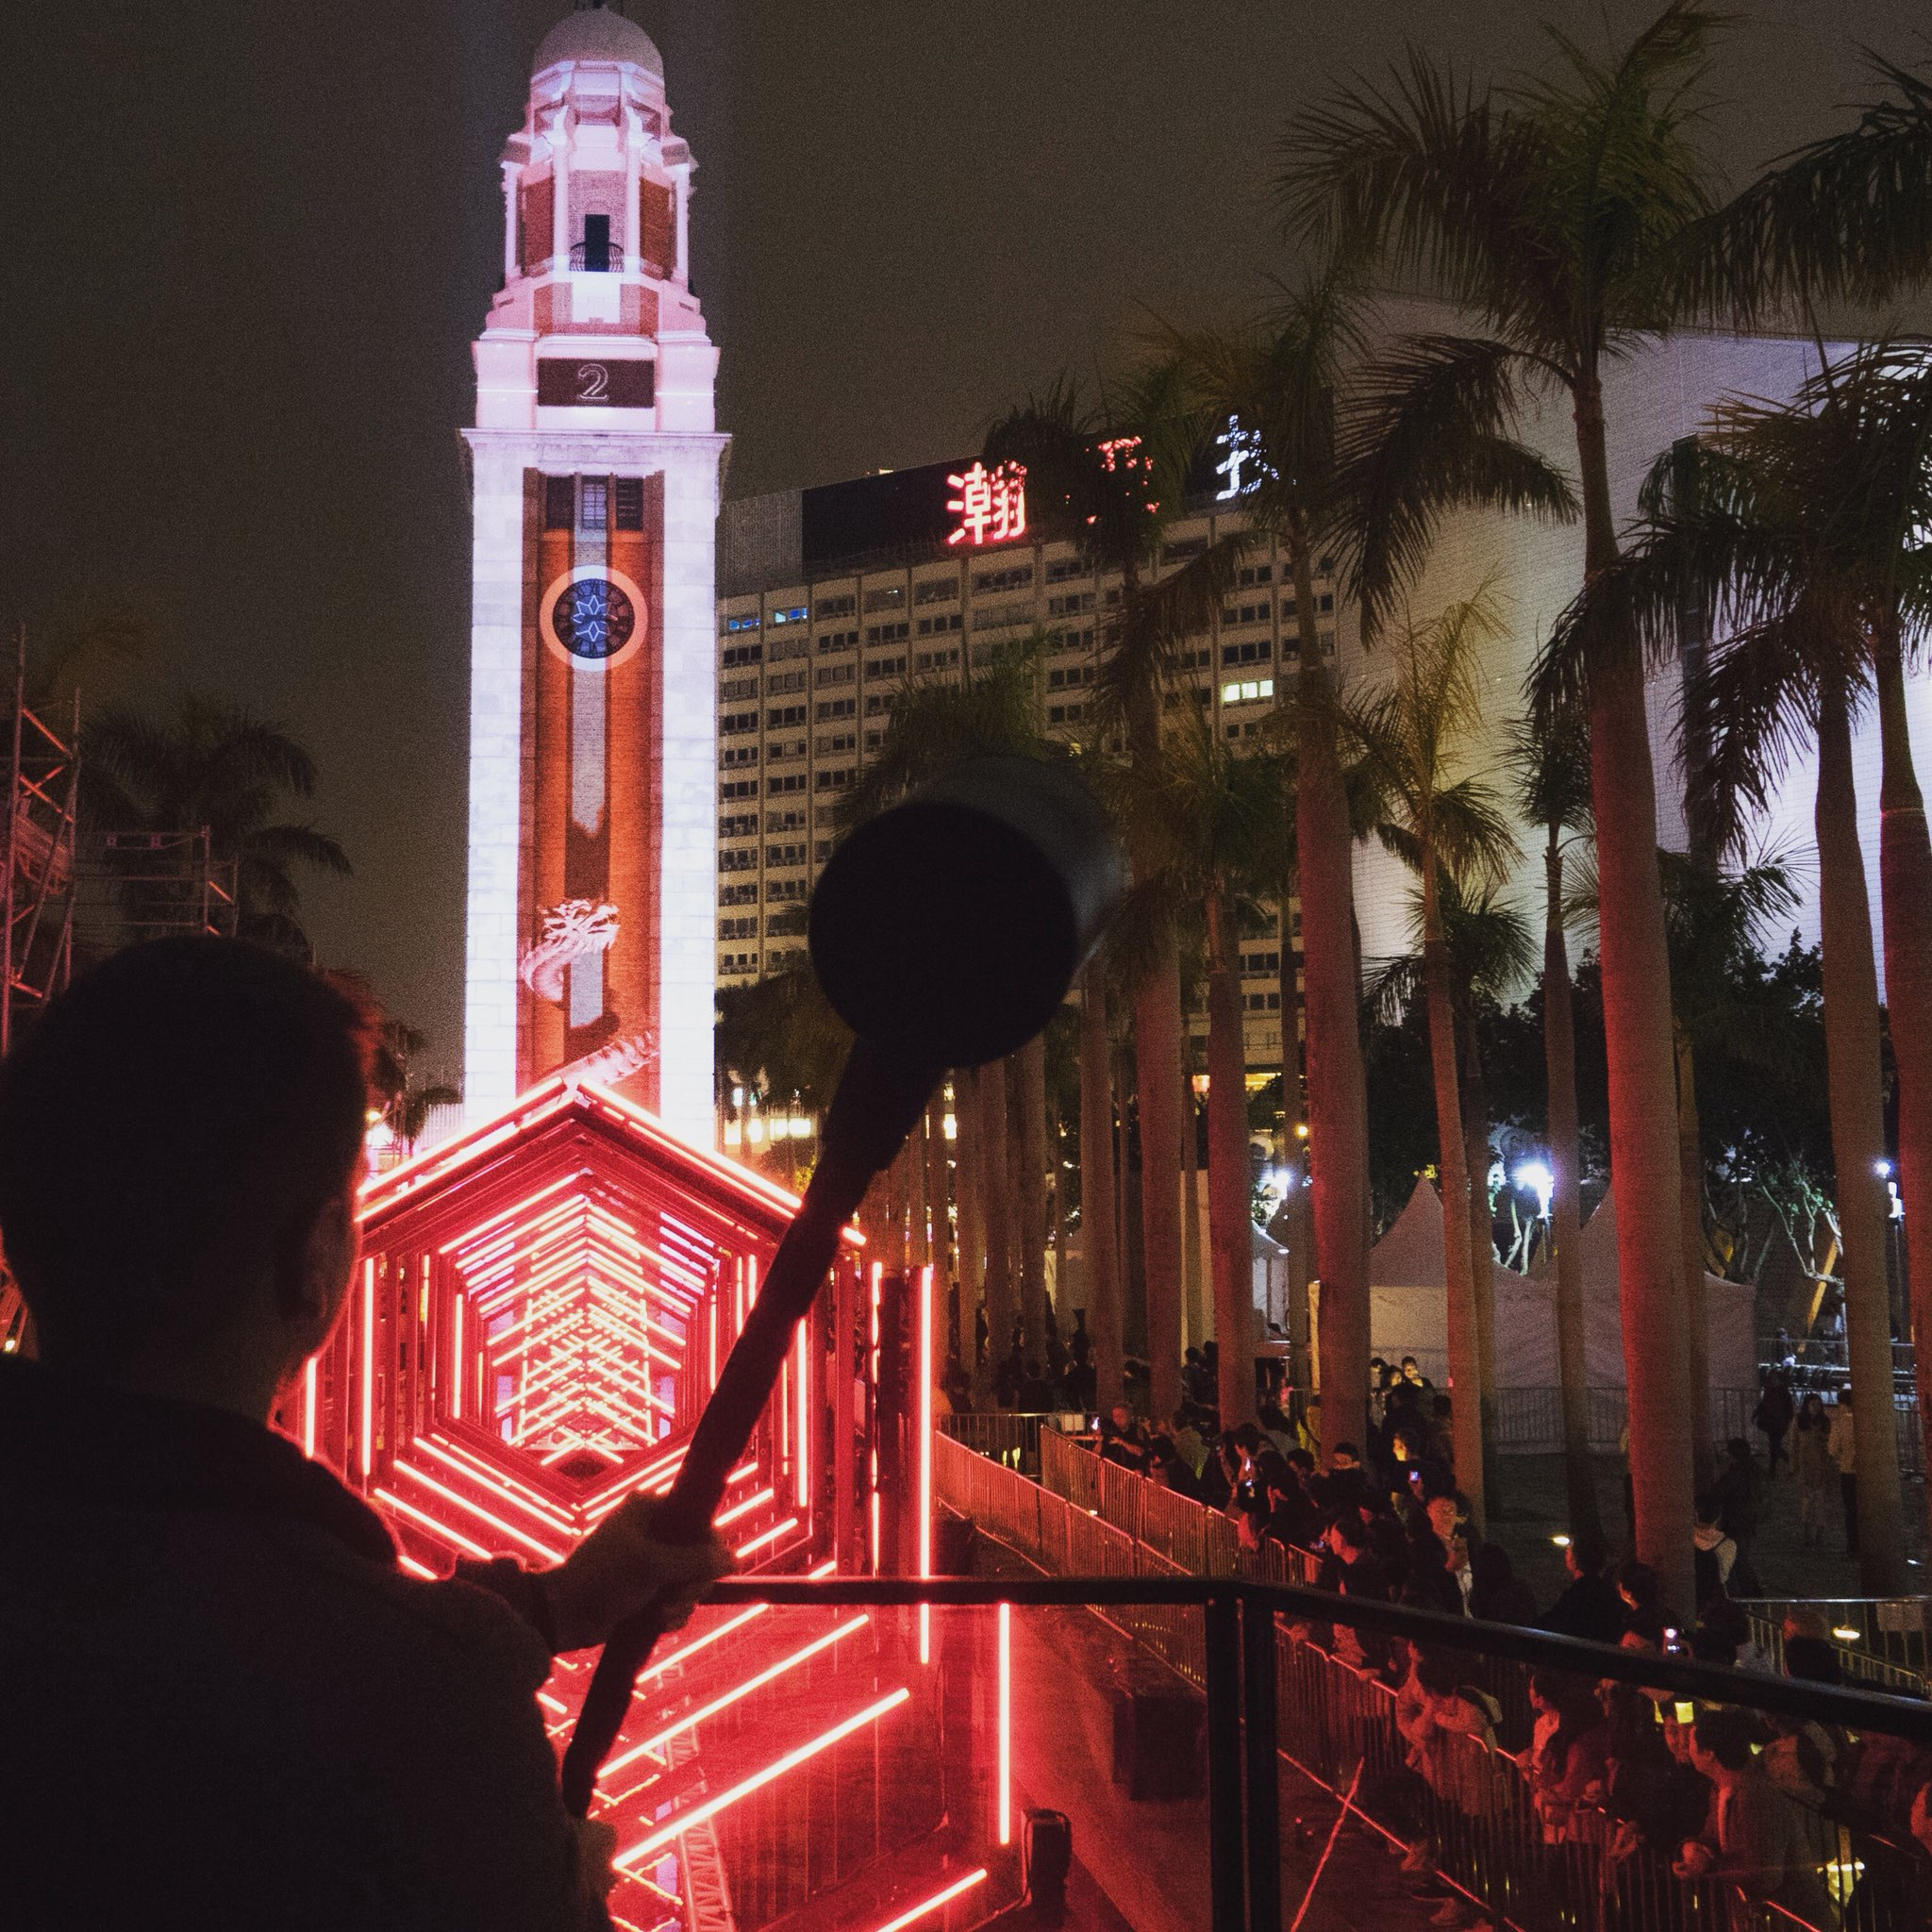
\includegraphics[scale=0.15]{img/long-striker.jpg}
    \caption{L'installation "Long Striker" à la fête des Lumières de Hong Kong}
\end{figure}

\clearpage

\subsubsection{Clients}

Les clients de LTBL et de Vendredi 4 sont, le plus souvent, de la région Rhône-Alpes, mais peuvent aussi être en région parisienne.
Ces clients sont des PME ou des grands groupes désirant de nouvelles installations interactives pour leurs showrooms.
Au travers de ces installations, ils peuvent montrer leur produit de manière esthétique à leurs clients.
Les showrooms ne sont pas les seuls installations organisées par LTBL, on retrouve aussi des présentations de produits pour les salons ou l'affichage de données pour la productivité.

\bigskip

Quelques clients :

\begin{multicols}{2}
    \begin{itemize}
        \item Biomérieux
        \item EDF
        \item Michelin
        \item Somfy
        \item Visiativ
        \item Courchevel
        \item Fête des Lumières
        \item Et bien d'autres \ldots
    \end{itemize}
\end{multicols}